\documentclass[10pt,paper=a4,final]{scrartcl}
\usepackage[utf8]{inputenc}
\usepackage{tabularx}		%used for the tables
\usepackage{geometry}		%allows us to specify the 'seitenrand'
\usepackage[table]{xcolor}	%allows us to make colored fields in the tables
\usepackage{graphicx}		%package used to include graphics
\usepackage{hyperref}   	%used to make klickable links
\usepackage{pdflscape}	%allows landscape mode
\usepackage{supertabular}
\usepackage{listings}
\lstset{language=python,
  basicstyle=\small, 
  keywordstyle=\color{blue!80!black!100}, 
  identifierstyle=, 
  commentstyle=\color{green!50!black!100}, 
  stringstyle=\ttfamily\color{red!80!black!100}, 
  breaklines=true, 
  numbers=left, 
  numberstyle=\small, 
  frame=single, 
  backgroundcolor=\color{blue!3} 
} 

\setcounter{tocdepth}{4}        %include paragraph in tableofcontents
\setcounter{secnumdepth}{5}     %also number the paragraphs

%\hypersetup{linktocpage}	%make the tableofcontent klickable
\hypersetup{
  colorlinks,
  citecolor=black,
  filecolor=black,
  linkcolor=black,
  urlcolor=black
}

\setcounter{tocdepth}{4}	%include paragraph in tableofcontents
\setcounter{secnumdepth}{5}	%also number the paragraphs

%These two lines will allow us to specify our own headers/footers
\usepackage{fancyhdr}
\pagestyle{fancy}
 \setlength{\parskip}{0pt}
 \setlength{\baselineskip}{0pt}

%The next three lines set the default font to Arial
%use 'getnonfreefonts arial-urw' to install uarial on Linux systems
\usepackage[T1]{fontenc}
\usepackage[scaled]{uarial}
\renewcommand*\familydefault{\sfdefault}

\geometry{a4paper, top=20mm, right=20mm, bottom=20mm, left=20mm}
\title{Projektf\"uhrungsbericht}
\author{Niklaus Hofer, Lukas Kn\"opfel, Kaleb Tschabold}
\date{\today}

%defining header and footer
\fancyhf{}	%delete default values
\setlength{\headwidth}{\textwidth}	%header and footer width equal the text width
\fancyhead[LE,LO]{
\includegraphics[scale=0.6]{header.png}}
\fancyhead[RE,RO]{ProjectExplorer}
\fancyfoot[CE,CO]{Speicherdatum: \today{}}
\fancyfoot[RE,RO]{\thepage}

\begin{document}
\maketitle
\newpage
\begin{tabularx}{\textwidth}{ r X }	%X fields are stretched over the whole space
  \textcolor{white}{{\bf Status}}\cellcolor{blue!80!} & In Arbeit/In Prüfung/ {\bf Abgeschlossen}\cellcolor{blue!20!} \\
\textcolor{white}{{\bf Projektname}}\cellcolor{blue!80!} & Projektexplorer\cellcolor{blue!20!} \\
\textcolor{white}{{\bf Projektleiter}}\cellcolor{blue!80!} & Lukas Kn\"opfel\cellcolor{blue!20!} \\
\textcolor{white}{{\bf Auftraggeber}}\cellcolor{blue!80!} & M. Frieden, GIBB\cellcolor{blue!20!} \\
\textcolor{white}{{\bf Autoren}}\cellcolor{blue!80!} & Kaleb Tschabold, Lukas Kn\"opfel, Niklaus Hofer\cellcolor{blue!20!} \\
\textcolor{white}{{\bf Verteiler}}\cellcolor{blue!80!} & Lukas Knöpfel, Kaleb Tschabolt, Niklaus Hofer\cellcolor{blue!20!}
\end{tabularx}
\newline
\newline
\newline
{\bf Änderungskontrolle, Prüfung, Genehmigung}
\newline

\begin{tabularx}{\textwidth}{l l X X}
\textcolor{white}{Version}\cellcolor{blue!80!} & \textcolor{white}{Datum}\cellcolor{blue!80!} & \textcolor{white}{Beschreibung, Bemerkung}\cellcolor{blue!80!} & \textcolor{white}{Name oder Rolle}\cellcolor{blue!80!} \\
\cellcolor{blue!20!} 1.0& \cellcolor{blue!20!} 08.02.2011 & Dokument schreiben \cellcolor{blue!20!} & Niklaus Hofer \cellcolor{blue!20!} \\
\end{tabularx}
\newline
\newline
\newline
{\bf Definitionen und Abkürzungen}
\newline

\begin{tabularx}{\textwidth}{l X}
\textcolor{white}{Begriff/ Abkürzung}\cellcolor{blue!80!} & \textcolor{white}{Bedeutung}\cellcolor{blue!80!} \\
CLI \cellcolor{blue!20!} & Command Line Interface\cellcolor{blue!20!} \\
GUI \cellcolor{blue!20!} & Graphical user interface \cellcolor{blue!20!} \\
DB \cellcolor{blue!20!} & Database\cellcolor{blue!20!} \\
KM \cellcolor{blue!20!} & Konfigurationsmanagement \cellcolor{blue!20!} \\
\end{tabularx}
\newline
\newline
\newline
\bibliographystyle{plain}
\bibliography{projektfuehrung}{}
\flushleft
\newpage
\tableofcontents
\newpage
\section{Zweck des Dokuemnts}
Zusammenfassung von Planung und Ergebnissen zu den fünf Projektführungsthemen.
\begin{itemize}
  \item Projektmanagement
  \item Risikomanagement
  \item Qualitätsmanagement
  \item Konfigurationsmanagement
  \item Projektmarketing
\end{itemize}
\section{Projektplan}
\newpage
\begin{landscape}
\begin{tabularx}{\textwidth}{ |p{4.0cm}|l|l|l|l|l|l|l|l|l|l|l|l|l|l|l|l|l|l|l|l|l|l|l| }
\cline{1-24}	%need to use cline, cuz hline did not stretch over the whole width...
\bf Aktivit\"at & PL Soll & PL Ist & KW 05 & 06 & 07 & 08 & 09 & 10 & 11 & 12 & 13 & 14 & 15 & 16 & 17 & 18 & 19 & 20 & 21 & 22 & 23 & 24 & 25 \\
\cline{1-24}
Initialisierung & 12 & 12 & & \cellcolor[gray]{0.7} & & & & & & & & & & & & & & & & & & & \\
\cline{1-24}
Voranalyse & 36 & 36 & & & \cellcolor[gray]{0.7} & \cellcolor[gray]{0.7} & \cellcolor[gray]{0.7} & & & & & & & & & & & & & & & & \\
\cline{1-24}
Konzept & 36 & 36 & & & & & & \cellcolor[gray]{0.7} & \cellcolor[gray]{0.7} & \cellcolor[gray]{0.7} & & & & & & & & & & & & & \\
\cline{1-24}
Realisierung & 48 & 192 \cellcolor{red!100!} & & & & & & & & & \cellcolor[gray]{0.7} & \multicolumn{3}{|c|}{Ferien \cellcolor{green!70!}} & \cellcolor[gray]{0.7} & \cellcolor[gray]{0.7} & \cellcolor[gray]{0.7} & & & & & & \\
\cline{1-24}
Einf\"uhrung & 24 & 24 & & & & & & & & & & & & & & & & \cellcolor[gray]{0.7} & \cellcolor[gray]{0.7} & & & & \\
\cline{1-24}
Reserve & 24 & - & & & & & & & & & & & & & & & & & & \cellcolor[gray]{0.7} & \cellcolor[gray]{0.7} & & \\
\cline{1-24}
Abschlussphase & 12 & 24 \cellcolor{red!100!} & & & & & & & & & & & & & & & & & & & & \cellcolor[gray]{0.7} & \cellcolor[gray]{0.7}\\
\cline{1-24}
\multicolumn{24}{|c|}{\bf Projektleiter} \\
\cline{1-24}
Niklaus Hofer & & & \cellcolor[gray]{0.7} & \cellcolor[gray]{0.7} & \cellcolor[gray]{0.7} & \cellcolor[gray]{0.7} & \cellcolor[gray]{0.7} & & & & & & & & & & & & & & & & \\
\cline{1-24}
Kaleb Tschabold & & & & & & & & \cellcolor[gray]{0.7} & \cellcolor[gray]{0.7} & \cellcolor[gray]{0.7} & \cellcolor[gray]{0.7} & \cellcolor[gray]{0.7} & \cellcolor[gray]{0.7} & \cellcolor[gray]{0.7} & \cellcolor[gray]{0.7} & & & & & & & & \\
\cline{1-24}
Lukas Kn\"opfel & & & & & & & & & & & & & & & & \cellcolor[gray]{0.7} & \cellcolor[gray]{0.7} & \cellcolor[gray]{0.7} & \cellcolor[gray]{0.7} & \cellcolor[gray]{0.7} & \cellcolor[gray]{0.7} & \cellcolor[gray]{0.7} & \cellcolor[gray]{0.7}\\
\cline{1-24}
\end{tabularx}
\end{landscape}
\newpage
\section{Projektbericht}
\subsection{KW 7}
\begin{description}
  \item {\bf Stand der Arbeit: } \\
    \begin{itemize}
      \item Nachforschungen zu verschidenen Technologien.
      \item Die Arbeiten am Voranalysebericht schreiten gut voran.
      \item Wir haben bereits ein recht gutes Bild der aktuellen Lage geschaffen und wissen in etwa, welche Produkte vergleichbares liefern.
    \end{itemize}
  \item {\bf Probleme und Fragen: } \\
    \begin{itemize}
      \item Zurzeit gibt es von unserer Seite her keine Fragen.
    \end{itemize}
  \item {\bf nächste Schritte: } \\
    \begin{itemize}
      \item Nächsten Dienstag werden wir die Anforderungen erarbeiten.
      \item Sobald wir uns zu den verschiedenen Technologien, die für das Projekt in Frage kommen informiert haben (voraussichtlich nächste Woche, hängt von den Vortschritten bei den Specs ab), werden wir die verschiedenen Möglichkeiten analysieren und vergleichen.
    \end{itemize}
\end{description}
\subsection{KW 8}
\begin{description}
  \item {\bf Stand der Arbeit: } \\
    \begin{itemize}
      \item Wir sind zur Zeit mit der Evaluierung der verschiedenen Varianten beschäftigt. Dabei sind die mit Ihnen bereits besprochenen Probleme aufgetaucht, die wir nun als nächsten Schritt lösen werden.
      \item Die Arbeit am Voranalysebericht schreitet ansonsten gut voran und ist beinahe abgeschlossen.
      \item Parallel zu dem neuen Dokument arbeiten wir zur Zeit auch an der Korrektur der alten Unterlagen.
    \end{itemize}
  \item {\bf Probleme und Fragen: } \\
    \begin{itemize}
      \item Zurzeit haben wir keine weiteren Fragen.
    \end{itemize}
  \item {\bf nächste Schritte: } \\
    \begin{itemize}
      \item Der nächste konkrete Schritt ist das Anpassen der Versionsanalyse.
      \item Ist die Voranalyse abgeschlossen wird das Dokument aufgeräumt (Rechtschreibung, Punktierung,\ldots) und dann mit LaTeX in die Reinversion geschrieben.
    \end{itemize}
\end{description}
\subsection{KW 9}
\begin{description}
  \item {\bf Stand der Arbeit: } \\
    \begin{itemize}
      \item Voranalysebericht fertig gestellt.
      \item Parallel zu den neuen Dokumenten arbeiten wir zur Zeit auch an der Korrektur der alten Unterlagen.
    \end{itemize}
  \item {\bf Probleme und Fragen: } \\
    \begin{itemize}
      \item Zurzeit haben wir keine weiteren Fragen.
    \end{itemize}
  \item {\bf nächste Schritte: } \\
    \begin{itemize}
      \item Erstellen des Konzeptberichtes.
    \end{itemize}
\end{description}
\subsection{KW 10}
\begin{description}
  \item {\bf Stand der Arbeit: } \\
    \begin{itemize}
      \item Ersellung des Konzeptberichts.
      \item Arbeit am Klassendiagram.
    \end{itemize}
  \item {\bf Probleme und Fragen: } \\
    \begin{itemize}
      \item Zurzeit haben wir keine weiteren Fragen.
    \end{itemize}
  \item {\bf nächste Schritte: } \\
    \begin{itemize}
      \item Die Arbeit am Konzepbericht wird noch eine Menge Arbeit beanspruchen. Besonders muessen viele Funktionen genau geplant und durchdacht werden.
    \end{itemize}
\end{description}
\subsection{KW 11}
\begin{description}
  \item {\bf Stand der Arbeit: } \\
    \begin{itemize}
      \item Ich(Kaleb) habe nun die Aufgabe des Projektleiters übernommen.
      \item Wir haben heute zum grossen Teil einige Prototypen erstellt.
      \item Auch haben wir unser Klassen-Diagramm überarbeitet.
    \end{itemize}
  \item {\bf Probleme und Fragen: } \\
    \begin{itemize}
      \item Zurzeit haben wir keine Fragen.
    \end{itemize}
  \item {\bf nächste Schritte: } \\
    \begin{itemize}
      \item Da wir mit unserem Konzept noch nicht weit sind, müssen wir jetzt vor allem zu Hause das Konzept erarbeiten.
      \item Besonders das Klassendiagramm wollen wir optimieren.
      \item Auch die kleinen Korrekturen von den vorherigen Dokumenten müssen wir noch nachführen(Projektantrag und Voranalyse).
    \end{itemize}
\end{description}
\subsection{KW 12}
\begin{description}
  \item {\bf Stand der Arbeit: } \\
    \begin{itemize}
      \item Wir haben gestern das Konzept abgeschlossen. Wir haben gemerkt, dass wir den Zeitplan nicht gut eingeteilt haben und darum sind wir gestern ein bisschen in Zeitdruck gekommen.
      \item Wir beginnen jetzt mit der Realisierung.
    \end{itemize}
  \item {\bf Probleme und Fragen: } \\
    \begin{itemize}
      \item Zurzeit haben wir keine Fragen.
    \end{itemize}
  \item {\bf nächste Schritte: } \\
    \begin{itemize}
      \item Wir werden nun nächstes Mal, die Aufteilung machen, in der definiert ist, wer welche Programmteile programmiert.
      \item In den Frühlingsferien haben wir dann Zeit um voll am Projekt zu arbeiten.
    \end{itemize}
\end{description}
\subsection{KW 13}
\begin{description}
  \item {\bf Stand der Arbeit: } \\
    \begin{itemize}
      \item Wir sind gerade dran richtig in die Realisierungsphase zu starten.
      \item Wir sind gerade dran alle Dateien und etc. zu erstellen, damit wir, dann die Funktionalitäten erstellen können.
    \end{itemize}
  \item {\bf Probleme und Fragen: } \\
    \begin{itemize}
      \item Zurzeit haben wir keine Fragen.
    \end{itemize}
  \item {\bf nächste Schritte: } \\
    \begin{itemize}
      \item Ich werde einen Zeitplan für die Unterrichtsfreiezeit machen so, dass wir gegen Ende dieser Phase nicht in Zeitdruck kommen.
      \item Wir müssen diese Zeit auch nutzen um unsere Dokumente(Voranlyse,\ldots) zu korrigieren.
      \item Auch die aktuellen Dokumente(Realisierungsbericht und Projektführungsbericht) ergänzen.
    \end{itemize}
\end{description}
\subsection{KW 17}
\begin{description}
  \item {\bf Stand der Arbeit: } \\
    \begin{itemize}
      \item Wir sind gerade voll dran am System entwickeln.
      \item Ich habe gerade heute Abend die erste Version zum Setzten und Suchen von Tags programmiert.
    \end{itemize}
  \item {\bf Probleme und Fragen: } \\
    \begin{itemize}
      \item Zurzeit haben wir keine Fragen.
    \end{itemize}
  \item {\bf nächste Schritte: } \\
    \begin{itemize}
      \item Wir müssen besprechen wer, was bis zum nächsten Meilenstein macht.
      \item Auch den Realisierungsbericht müssen wir anfangen zu erstellen.
    \end{itemize}
\end{description}
\subsection{KW 18}
\begin{description}
  \item {\bf Stand der Arbeit: } \\
    \begin{itemize}
      \item Ich (Lukas) habe nun die Aufgabe des Projektleiters übernommen.
      \item Wir haben eine experimentelle Version unseres Programmes die schon einige Grundfunktionen integriert hat.
    \end{itemize}
  \item {\bf Probleme und Fragen: } \\
    \begin{itemize}
      \item Zurzeit haben wir keine Fragen.
    \end{itemize}
  \item {\bf nächste Schritte: } \\
    \begin{itemize}
      \item Wir werden hauptsächlich am Programm arbeiten.
      \item Aus Zeitmangel werden wir uns auf die Linux Version unseres Programmes konzentrieren. Die Windows und Mac Versionen werden je nachdem auf wieviele Probleme wir stossen weniger Funktionalität besitzen als die Linux Version.
    \end{itemize}
\end{description}
\subsection{KW 20}
\begin{description}
  \item {\bf Stand der Arbeit: } \\
    \begin{itemize}
      \item Wir haben eine stabile Version unseres Programmes auf Linux.
      \item Wir haben uns einen Überblick über das Projekt verschafft. Wir wissen nun welche Funktionen funktionieren und welche eine Überarbeitung benötigen.
    \end{itemize}
  \item {\bf Probleme und Fragen: } \\
    \begin{itemize}
      \item Zurzeit haben wir keine Fragen.
    \end{itemize}
  \item {\bf nächste Schritte: } \\
    \begin{itemize}
      \item Wir werden alle Funktionen in das GUI implementieren, damit wir sie an der Präsentation zeigen können.
      \item Ausserdem werden wir das Programm noch vollständig auf Windows portieren und eine Versionierung einbauen.
      \item Wir bereiten uns auch auf die Präsentation vor, da diese nun vorverschoben wurde.
    \end{itemize}
\end{description}
\subsection{KW 21}
\begin{description}
  \item {\bf Stand der Arbeit: } \\
    \begin{itemize}
      \item Wir arbeiten an der Präsentation um diese wie vereinbart nächsten Dienstag Vorzutragen.
    \end{itemize}
  \item {\bf Probleme und Fragen: } \\
    \begin{itemize}
      \item Zurzeit haben wir keine Fragen.
    \end{itemize}
  \item {\bf nächste Schritte: } \\
    \begin{itemize}
      \item Wir werden die Präsentation fertigstellen.
      \item Wir werden uns absprechen um im vorgegebenen Zeitrahmen zu bleiben.
      \item Wir werden eine dedizierte Maschine aufsetzen um unser Tool zu demonstrieren.
    \end{itemize}
\end{description}
\section{Risikokatalog}
\begin{tabularx}{\textwidth}{|l|X|X|X|p{1cm}|}
  \hline
  \bf Nr. \cellcolor{blue!20!}& \bf Risiko f\"ur das Projekt \cellcolor{blue!20!}& \bf m\"ogliche Auswirkungen \cellcolor{blue!20!}& \bf Massnahmen \cellcolor{blue!20!}& \bf Status \cellcolor{blue!20!}\\ \hline
  1. & Die ausgew\"ahlten Technologien sind f\"ur die Programmierung der Applikation nicht geeignet, da Funktionen fehlen oder aufwendig zu implementieren sind.& Die Arbeit an den einzelnen Teilen des Programmes wird massiv aufwendiger. Versp\"atungen k\"onnen nicht ausgeschlossen werden. Evtl. m\"ussten sogar Teile der Applikation mit einer anderen Technologie neu geschriben werden.& Genaue Nachforschungen zu den Technologien anstellen. Prototypen und kleine Testapplikationen entwickeln.& erledigt\\ \hline
  2. & Die Applikation kann nicht rechtzeigit fertiggestellt werden, da zu viele Funktionen geplant sind, die Implementierung Probleme macht oder Mitglieder des Teams ausfallen.& Das Projekt kann nicht rechtzeitig fertiggestellt werden. Die Qualit\"at der Applikation leidet.& Planen der Ressourcen.& erledigt\\ \hline
  3. & Die Kompatibilit\"at mit allen Betriebssystemen kann nicht gew\"ahrleistet werden, da manche features auf einer Plattform viel schwieriger zu implemntieren sind als auf einer anderen.& Das Programm l\"auft nicht auf allen Systemen gleich stabil. M\"oglicherweise sind auch einige Funktionen nicht auf allen Plattformen verf\"ugbar. Zeitaufwendige Implementierung f\"ur verschidene Plattformen k\"onnten auch zu Versp\"atungen f\"uhren.& Verwendung einer Systemunabh\"angigen Sprache (Python). Nachvorschungen anstellen zu den Modulen, die f\"ur die Funktionalit\"at entscheidend sind. Im schlimmsten Falle k\"onnten wir auch den Support f\"ur eine Plattform fallen lassen.& erledigt\\ \hline
  4. & Die Applikation gen\"ugt den Anspr\"uchen in Sachen Stabilit\"at, Nutzerfreundlichkeit oder einem anderen Gebiet nicht.& Die Applikation funktioniert nicht wie gew\"unscht.& Die einzelnen Komponenten, ihre interoperabilit\"at und integration sowie das fertige Produkt sind zu testen& erledigt\\ \hline
\end{tabularx}
\section{QS-Plan}
\subsection{Vorgehen zur Qualitätssicherung}
Die Qualit\"at der Applikation haben wir durch Tests sichergestellt. Code-reviews haben keine stattgefunden.\\
Zum Testen der Applikation kamen vorallem Modultests zum Einsatz. Genauere Details zur Durchf\"uhrung der Tests k\"onnen \cite[4. Systemtests]{realisierung} entnommen werden.

Die Dokumente wurden jeweils nach dem Erstellen durchgelesen. Die Struktur der Vorlagedokumente gab jeweils vor, welche Informationen enthalten sein mussten.
\subsection{Qualitätsziele}
\newpage
\begin{tabularx}{\textwidth}{|l|l|X|X|}
  \hline
  \bf Nr. \cellcolor{blue!20!}& \bf Qualit\"atsmerkmal \cellcolor{blue!20!}& \bf Qualit\"atsziel \cellcolor{blue!20!}& \bf besondere QS-Massnahmen um das Ziel zu erreichen \cellcolor{blue!20!}\\ \hline
  \multicolumn{4}{|c|}{\bf aus Benutzersicht} \\ \hline
  1 & Funktionserf\"ullung & Die Applikation soll die im Konzeptbericht \cite{konzept} festgelegten Ziele erf\"ullen. & - \\ \hline
  2 & Effizienz & Die Applikation soll z\"ugig reagieren, die Benutzung soll sich durchgehen schnell anf\"hlen.& Evtl. m\"ussen einzelne Teil des Codee auf Geschwindigkeit optimiert werden.\\ \hline
  3 & Zuverl\"assigkeit& Die Applikation soll auch bei falschen Eingaben oder schnellen Eingabe-Abfolgen zuverl\"assig funktionieren und darf nicht abst\"urzen.& Die Tests sehen auch ungew\"ohnliche Szenarien vor, die die Applikation stark belasten und in dieser Form im Alltag nicht zu erwarten sind.\\ \hline
  4 & Benutzbarkeit& Die Oberfl\"ache des Programmes soll intuitiv sein. Wo das nicht direkt m\"oglich ist, soll sich die Applikation an gewohnte Bedienungs-Paradigmen halten.& - \\ \hline
  5 & Sicherheit& Die Applikation soll die Sicherheit und integrit\"at der Benutzerdaten nicht gef\"ahrden.& \\ \hline
  \multicolumn{4}{|c|}{\bf aus Entwicklersicht} \\ \hline
  6 & Erweiterbarkeit & Die Applikation wird objektorientiert entwickelt. Die Klassen werden systematisch und eindeutig bennt. Zudem sind die Funktionen fehlertollerant aufgebaut. Funktionen die von aussen genutzt werden k\"onnen enthalten eine Erl\"auterung.& - \\ \hline
  7 & Wartbarkeit & Die Applikation ist ausreichend dokumentiert. Ablaeufe sind direkt im Code dokumentiert, komplexe Vorg\"ange sind in der Dokumentation erkl\"art.& - \\ \hline
  8 & \"Ubertragbarkeit & - & - \\ \hline
  9 & Wiederverwendbarkeit & Die Komponenten der Applikation h\"ange nicht fest voneinander ab. Einzelne Komponenten (z.B. das Backend) k\"onnen auch in anderen Projekten wiederverwendet werden.& - \\ \hline
  \multicolumn{4}{|c|}{\bf Projektf\"uhrung} \\ \hline
  10 & Kommunikation der Beteiligten & Die Entwickler sprechen sich untereinander ab, damit nicht aneinander vorbeiprogrammiert ist. Treten Fragen zum Code eine anderen Mitgliedes des Teams auf, so k\"onnen diese gestellt werden.& - \\ \hline
  12 & Termineinhaltung & Die Termine aus dem Projektplan (siehe oben) werde eingehalten.& - \\ \hline
  13 & Projekdokumentation & Die Vorgegebenen Dokumente werden p\"unktlich eingereicht. Mails die zwischen den Entwicklern ausgetauscht werden werden aufgehoben.& - \\ \hline
\end{tabularx}
\subsection{Pr\"ufplan}
\begin{tabularx}{\textwidth}{|l|l|l|l|X|X|}
  \hline
  \bf Pr\"ufobjekt \cellcolor{blue!20!}& \bf Termin \cellcolor{blue!20!}& \bf Pr\"ufer \cellcolor{blue!20!}& \bf Pr\"ufmethode \cellcolor{blue!20!}& \bf Pr\"ufkriterien \cellcolor{blue!20!}& \bf Bemerkungen \cellcolor{blue!20!}\\ \hline
  Projektantrag		& & Lehrperson & Review & Alle Punkte behandelt (nach Vorlage), Rechtschreibung & \\ \hline
  Projektplan		& & Lehrperson & Review & Alle Punkte behandelt (nach Vorlage), Rechtschreibung, Tabelle ausgef\"ullt& \\ \hline
  Voranalysebericht	& & Lehrperson & Review & Alle Punkte behandelt (nach Vorlage), Rechtschreibung, Diagramme vorhanden, Auswertungen vorhanden & \\ \hline
  Konzeptbericht	& & Lehrperson & Review & Alle Punkte behandelt (nach Vorlage), Rechtschreibung, Diagramme vorhanden, Anwendungsf\"alle beschrieben, Klassendiagram vorhanden, DB-Schema vorhanden & \\ \hline
  Programm		& & Lehrperson & Tests & siehe \cite[4. Systemtests]{realisierung} & \\ \hline
  Realisierungsbericht	& & Lehrperson & Review & Alle Punkte behandelt (nach Vorlage), Rechtschreibung, Klassendiagram aktuell, DB-Schema aktuell, Benutzerhandbuch vorhanden, Supporthandbuch vorhanden, Tests erl\"autert, Code im Dokument & \\ \hline
  Einf\"uhrungsbericht	& & Lehrperson & Review & Alle Punkte behandelt (nach Vorlage), Rechtschreibung & \\ \hline
  Projektf\"uhrung	& & Lehrperson & Review & Alle Punkte behandelt (nach Vorlage), Rechtschreibung & \\ \hline
\end{tabularx}
\subsection{Pf\"ufmethoden}
\subsubsection{Review}
Die Dokumente wurden jeweils durchgelesen von mindestens einem Teammitglied. Zudem wurde beim Erstellen eine Rechtschreibekorrektur eingesetzt.
\subsubsection{Applikations-Tests}
siehe \cite[4. Systemtests]{realisierung} 
\subsection{Pr\"ufspezifikationen}
\subsubsection{Checklisten für die Prüfung der Projektdokumente}
\paragraph{Projektantrag}
\begin{tabularx}{\textwidth}{|l|X|X|}
  \hline
  {{\bf Nr.}}\cellcolor{blue!20!} & {\bf Pr\"ufkriterium}\cellcolor{blue!20!} & {\bf Pr\"ufergebnis, Bemerkungen}\cellcolor{blue!20!} \\ \hline
  1 & Rechtschreibung & ist nicht erfolgt \\ \hline
  2 & Alle Punkte behandelt & erf\"ullt \\ \hline
\end{tabularx}
\paragraph{Projektplan}
\begin{tabularx}{\textwidth}{|l|X|X|}
  \hline
  {{\bf Nr.}}\cellcolor{blue!20!} & {\bf Pr\"ufkriterium}\cellcolor{blue!20!} & {\bf Pr\"ufergebnis, Bemerkungen}\cellcolor{blue!20!} \\ \hline
  1 & Rechtschreibung & ist nicht erfolgt \\ \hline
  2 & Alle Punkte behandelt & erf\"ullt \\ \hline
  3 & Tabelle ausgef\"ullt & erf\"ullt \\ \hline
\end{tabularx}
\paragraph{Voranalysebericht}
\begin{tabularx}{\textwidth}{|l|X|X|}
  \hline
  {{\bf Nr.}}\cellcolor{blue!20!} & {\bf Pr\"ufkriterium}\cellcolor{blue!20!} & {\bf Pr\"ufergebnis, Bemerkungen}\cellcolor{blue!20!} \\ \hline
  1 & Rechtschreibung & erf\"ullt \\ \hline
  2 & Alle Punkte behandelt & erf\"ullt \\ \hline
  3 & Diagramme vorhanden & erf\"ullt \\ \hline
  4 & Auswertungen vorhanden & erf\"ullt \\ \hline
\end{tabularx}
\paragraph{Konzeptbericht}
\begin{tabularx}{\textwidth}{|l|X|X|}
  \hline
  {{\bf Nr.}}\cellcolor{blue!20!} & {\bf Pr\"ufkriterium}\cellcolor{blue!20!} & {\bf Pr\"ufergebnis, Bemerkungen}\cellcolor{blue!20!} \\ \hline
  1 & Rechtschreibung & erf\"ullt \\ \hline
  2 & Alle Punkte behandelt & erf\"ullt \\ \hline
  3 & Diagramme vorhanden & erf\"ullt \\ \hline
  4 & Anwendungsf\"alle beschrieben & erf\"ullt \\ \hline
  5 & Klassendiagram vorhanden & erf\"ullt \\ \hline
  6 & DB-Schema vorhanden & erf\"ullt \\ \hline
\end{tabularx}
\paragraph{Programm}
siehe \cite[4. Systemtests]{realisierung} 
\paragraph{Realisierungsbericht}
\begin{tabularx}{\textwidth}{|l|X|X|}
  \hline
  {{\bf Nr.}}\cellcolor{blue!20!} & {\bf Pr\"ufkriterium}\cellcolor{blue!20!} & {\bf Pr\"ufergebnis, Bemerkungen}\cellcolor{blue!20!} \\ \hline
  1 & Rechtschreibung & hat nicht stattgefunden\\ \hline
  2 & Alle Punkte behandelt & erf\"ullt\\ \hline
  3 & Klassendiagram aktuell& erf\"ullt \\ \hline
  4 & DB-Schema aktuell& erf\"ullt \\ \hline
  5 & Benutzerhandbuch vorhanden& erf\"ullt \\ \hline
  6 & Supporthandbuch vorhanden& erf\"ullt \\ \hline
  7 & Tests erl\"autert& erf\"ullt \\ \hline
  8 & Code im Dokument& erf\"ullt \\ \hline
\end{tabularx}
\paragraph{Einf\"uhrungsbericht}
\begin{tabularx}{\textwidth}{|l|X|X|}
  \hline
  {{\bf Nr.}}\cellcolor{blue!20!} & {\bf Pr\"ufkriterium}\cellcolor{blue!20!} & {\bf Pr\"ufergebnis, Bemerkungen}\cellcolor{blue!20!} \\ \hline
  1 & Rechtschreibung & erf\"ullt \\ \hline
  2 & Alle Punkte behandelt & erf\"ullt \\ \hline
\end{tabularx}
\paragraph{Projektf\"uhrung}
\begin{tabularx}{\textwidth}{|l|X|X|}
  \hline
  {{\bf Nr.}}\cellcolor{blue!20!} & {\bf Pr\"ufkriterium}\cellcolor{blue!20!} & {\bf Pr\"ufergebnis, Bemerkungen}\cellcolor{blue!20!} \\ \hline
  1 & Rechtschreibung & erf\"ullt \\ \hline
  2 & Alle Punkte behandelt & erf\"ullt\\ \hline
\end{tabularx}
\subsubsection{Testfalltabellen}
Testf\"alle wurden nur f\"ur den Code erstellt, nicht aber f\"ur die Dokumente. Die vertige Tabelle der Programmtests zusammen mit den Ergebnissen kann im Realisierungsbericht \cite{realisierung}eingesehen werden.

Die Testcases der Modultests (Unittests) k\"onnen im Code nachgesehen werden. Diese haben zum Teil komplexe Abh\"angigkeiten und pr\"ufen einige Funktionen mehrmals oder auf \"uberfl\"ussige Weise.
\begin{tabularx}{\textwidth}{|l|X|X|}
\hline
\bf Nr. \cellcolor{blue!20!}& \bf Anwendungsfall \cellcolor{blue!20!} & \bf Bemerkungen \cellcolor{blue!20!} \\ \hline
1 & Tag zu einer Datei hinzuf\"ugen. & Wahlweise eines das noch nicht oder schon vorhanden ist. \\ \hline
2 & Programm starten& \\ \hline
3 & Tag mit Sonderzeichen erstellen & Hat zu gewissen Punkten in der Entwicklung zu Problemen gef\"uhrt. \\ \hline
4 & CLI starten und testten. & Wird nicht erfolgen, da nicht umgesetzt. \\ \hline
5 & Tags zu einer bestimmten Datei anzeigen. & Geschieht durch das Selektieren der Datei. \\ \hline
6 & Verzeichnis das eine Datei mit Sonderzeichen im Namen enthält wird geöffnet und der Datei ein Tag hinzugefügt.& War vor den \"Anderungen am DB-Modul nicht m\"oglich. \\ \hline
7 & Alle Dateien eines Tags archivieren/versionieren. & \\ \hline
8 & Ansicht zwischen hierarchisch und tag-view wechseln.& Dazu gibt es zwei M\"oglichkeiten. \\ \hline
9 & Backup einer Datei anlegen.& \\ \hline
10 & Datei L\"oschen und die Reaktion vom Filesystem-Listener pr\"ufen.& der FS-Listener sollte eine entsprechende \"Anderung in der Datenbank machen.\\ \hline
11 & Datei anlegen  und die Reaktion vom Filesystem-Listener pr\"ufen.& \\ \hline
\end{tabularx}
\section{Konfigurationsmanagementplan (KM-Plan)}
\subsection{Aufzubewahrende Projektergebnisse und ggf. sonstige Dokumente}
Alle Ergebnisse k\"onnen auf Google Code abgerufen werden. \url{https://code.google.com/p/project-browser/source/browse/#svn}
\subsection{Ablagestruktur}
\begin{figure}[h!]
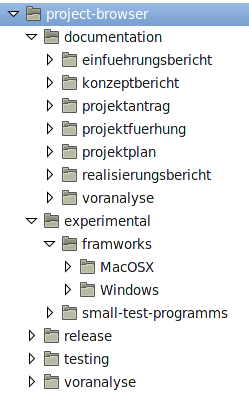
\includegraphics[scale=0.6]{tree.png}
\caption{Ablagestruktur}
\end{figure}
\subsubsection{documentation}
Alle Elemente der Dokumentation sind im Unterordner "documentation" abgelegt. Dort ist f\"ur jedes der Dokumente ein eigener Unterordner abgelegt, der jeweils den Namen des Dokumentes tr\"agt. In diesem Unterordner liegen alle Dateien, die zum Kompilieren des \LaTeX Dokuments nach PDF notwendig sind, sowie eine kompilierte Version als PDF.
\subsubsection{Code}
Der Code ist im Unterordner experimental abgelegt. Im weiteren Verlauf war die Verschiebung nach "testing" und sp\"ater nach "release" vorgesehen. In der Praxis hat das aber nie stattgefunden.

Die Python-files liegen direkt im experimental Ordner.\\
Dieser enth\"alt zudem einen Unterordner "frameworks", in dem weitere Installationsdateien liegen, die zur Benutzung des Programmes unter Windows oder MAC OS X ben\"otigt werden.
\subsection{Namenskonventionen}
Die Elemente der Dokumentation wurden jeweils gleich benannt wie in den verf\"ugbaren Vorlagen, also nach der aktuellen Projektphase.

Die Code-Files wurden nach dem Klassennamen benannt. Diese wiederum wurden nach den Aufgaben der Klassen vergeben.
\section{Konfigurationsidentifikation}
\subsection{Dokumentation}
\begin{tabularx}{\textwidth}{|l|l|X|}
\hline
 \bf Ergebniss \cellcolor{blue!20!}& \bf Status \cellcolor{blue!20!}& \bf Bemerkungen \cellcolor{blue!20!} \\ \hline
Projektantrag & fertig \cellcolor{green} & PDF File\\ \hline
Projektplan & fertig \cellcolor{green}& PDF File \\ \hline
Konzeptbericht & fertig \cellcolor{green}& PDF File \\ \hline
Voranalysebericht & fertig \cellcolor{green}& PDF File \\ \hline
Realisierungsbericht & fertig \cellcolor{green}& PDF File \\ \hline
Einf\"uhrungsbericht & fertig \cellcolor{green}& PDF File \\ \hline
Projektf\"uhrungsbericht & fertig \cellcolor{green}& PDF File \\ \hline
\end{tabularx}
\subsection{Applikation (sourcecode)}
\begin{tabularx}{\textwidth}{|l|l|X|}
\hline
 \bf Ergebniss \cellcolor{blue!20!}& \bf Status \cellcolor{blue!20!}& \bf Bemerkungen \cellcolor{blue!20!} \\ \hline
CLI.py & in Arbeit/nicht fertig \cellcolor{red}& Command line interface f\"ur das Programm.\\ \hline
Constant.py & fertig \cellcolor{green}& Enth\"alt Werte die zur Laufzeit vom Programm ben\"otigt werden, sich aber nicht ver\"andern. \\ \hline
DB.py & fertig \cellcolor{green}& Dient als Schnittstelle zur Datenbank \\ \hline
File.py & fertig \cellcolor{green}& Repr\"asentiert eine Datei auf dem Dateisystem und wird innerhalb der Applikation zum Informationsaustausch verwendet. \\ \hline
FileManager.py & fertig \cellcolor{green}& Dateimanager Funktionen. \\ \hline
FileProperties.py & fertig \cellcolor{green}& Dient zum Setzen von Tags. \\ \hline
FileSystemListener.py & fertig \cellcolor{green}& Mutterklasse der Dateisystem-Listener. \\ \hline
FileSystemListener\_Linux.py & fertig \cellcolor{green}& Filesystem-Listener-variante f\"ur Linux. \\ \hline
FileSystemListener\_Mac.py & in Arbeit/nicht fertig \cellcolor{red}& Filesystem-Listener-variante f\"ur MAC OS X. \\ \hline
FileSystemListener\_Windows.py & in Arbeit/nicht fertig \cellcolor{red}& Filesystem-Listener-variante f\"ur Windows. \\ \hline
GUI.py & fertig \cellcolor{green}& Stellt das GUI dar. \\ \hline
HirarchicalView.py &  fertig \cellcolor{green}& Hierarchische Darstellung der Dateien. Erbt von View.\\ \hline
Main.py & fertig \cellcolor{green}& Startpunkt der Applikation. \\ \hline
RepeatTimer.py & in Arbeit/nicht fertig \cellcolor{red}& Backups in regelm\"assigen Zeitabst\"anden wiederholen. \\ \hline
TagManager.py & fertig \cellcolor{green}& Handeln der Tags. \\ \hline
TagView.py & fertig \cellcolor{green}& Darstellung der Dateien nach Tags. Erbt von View. \\ \hline
Utility.py & fertig \cellcolor{green}& Enth\"alt kleine Funktionen die an verschiedenen Stellen wiederverwendet werden. \\ \hline
View.py & fertig \cellcolor{green}& Mutterklasse f\"ur die verschiedenen Views. \\ \hline
gui.glade & fertig \cellcolor{green}& XML Datei. Beschreibt die GTK Oberfl\"ache \\ \hline
fileproperties.glade & fertig \cellcolor{green}& XML Datei. \\ \hline
\end{tabularx}
\end{document}
